\documentclass[11pt,fleqn, a4paper]{exam}
\usepackage[utf8]{inputenc}

\usepackage[margin=1in]{geometry}
\usepackage{amsmath,amssymb}
\usepackage{gensymb}
\usepackage{multicol}
\usepackage{float}
\usepackage{graphicx}
\usepackage{units,icomma}
\usepackage{hyperref}
\usepackage{enumerate}
\usepackage{wasysym}
\usepackage{multirow}
\usepackage[usenames,dvipsnames]{xcolor}
\usepackage[margin=1.5cm]{caption}
%\everymath{\displaystyle}

\hyphenation{
  chro-no-ampe-ro-met-ric
  ber-dia-me-ter
  de-ngan
  me-nem-pati
  mic-ro-graphs
  ka-langan}

\renewcommand{\figurename}{Gambar.}
\renewcommand{\labelitemi}{$-$}


\newcommand{\class}{OLIMPIADE ASTRONOMI}
\newcommand{\term}{Tingkat Provinsi - 2016}
\newcommand{\examnum}{OSP Astronomi 2016}
%\newcommand{\examdate}{11/02/2014}
%\newcommand{\timelimit}{120 Minutes}

\pagestyle{head}
\firstpageheader{}{}{}
\runningheader{\examnum}{}{Halaman \thepage\ dari \numpages}
\runningheadrule


\begin{document}

\noindent
\begin{tabular*}{\textwidth}{l @{\extracolsep{\fill}} r @{\extracolsep{6pt}} l}
\textbf{\class} \\% & \textbf{Name:} & \makebox[2in]{\hrulefill}\\
\textbf{\term}  %&&\\
%\textbf{\examnum} &&\\
%\textbf{\examdate} &&\\
%\textbf{Time Limit: \timelimit} & Teaching Assistant & \makebox[2in]{\hrulefill}
\end{tabular*}\\
\rule[2ex]{\textwidth}{2pt}

\noindent
\begin{tabular}{ll}
\textit{Copyright} (c) 2016 & Ridlo W. Wibowo (ridlo.w.wibowo@gmail.com)\\
                   & Sulistiyowati (sulis.astro08@gmail.com)
\end{tabular}

\vspace{0.3cm}
\noindent
Solusi ini dibuat tanpa jaminan kesesuaian dengan solusi resmi dari juri olimpiade sains bidang Astronomi. Pengguna boleh menyebarluaskan dan/atau memodifikasi solusi ini dengan mencantumkan sumber asli. Hak cipta soal ada pada Kementerian Pendidikan dan Kebudayaan dan dilindungi undang-undang.

\vspace{0.4cm}
\noindent
\rule[2ex]{\textwidth}{1.5pt}

\textbf{Soal Pilihan Ganda}

\begin{questions}
\question Perbedaan utama antara lensa dan cermin sebagai pengumpul cahaya dalam sistem teleskop adalah
\begin{choices}
\choice Panjang fokus lensa bergantung pada panjang gelombang, sedangkan cermin tidak
\choice Panjang fokus cermin bergantung pada panjang gelombang, sedangkan lensa tidak
\choice Cermin berbentuk cembung, sedangkan lensa harus berbentuk cekung
\choice Objek tidak dapat ditegakkan dengan kedua sistem pengumpul cahaya ini
\choice Membuat cermin lebih mudah daripada membuat lensa untuk pengumpul cahaya
\end{choices}

\textit{Jawaban: A} atau \textit{E*}\\
\textit{Aberasi khromatis}\\
Lensa mengalami aberasi khromatis, menyebabkan panjang gelombang yang berbeda memiliki fokus yang sedikit berbeda. Hal ini terjadi karena cahaya polikromatis melewati dua medium yang berbeda, sedangkan kecepatan cahaya berubah ketika melewati suatu medium bergantung pada panjang gelombangnya (menyebabkan indeks refraksi berbeda untuk setiap panjang gelombang). Pada cermin, cahaya tidak melewati medium yang berbeda (atau melewati hanya sedikit) sehingga aberasi khromatis bisa dibilang tidak ada.

\textit{Mana yang lebih susah untuk dibuat, cermin atau lensa?} \\
Untuk pengumpul cahaya (teleskop) \textit{berukuran besar} maka dengan teknologi saat ini membuat cermin lebih mudah. Untuk lensa perlu bahan yang bisa meneruskan sebanyak mungkin gelombang elektromagnetik dan tanpa cacat dalam pembuatannya (gelembung, dlsb). Kita perlu menghaluskan kedua sisi lensa. Sedangkan cermin hanya perlu menghaluskan satu sisi bahan dan memberi pelapis perak atau alumunium (terkadang ditambah lapisan lain sesuai kebutuhan). Tidak hanya itu, untuk menyangga lensa berukuran besar sangatlah susah karena hanya sisinya yang tipis yang boleh di``sentuh'', sedangkan cermin dapat kita ``taruh'' begitu saja di sisi yang tidak dilapisi. 

Diperkirakan 4000 S.M. cermin sudah dibuat walaupun tanpa proses ``coating'', sedangkan lensa sudah digunakan 700 S.M., walaupun demikian teleskop  pertama dibuat menggunakan lensa, kamera kita dibuat dengan lensa, mengapa? 
Teleskop reflektor butuh meletakkan cermin pemantul dibagian depan teleskop.  Hal ini tentu tidak mudah dan tidak efisien untuk teleskop berukuran sangat kecil (juga kamera). Jadi untuk masa sekarang semuanya punya tantangan masing-masing karena kebutuhan yang berbeda, susah untuk memilih mana yang lebih sulit dibuat.


\vspace{0.5cm}
\question Pada tanggal 17 Januari 2016, komet Catalina berada pada posisi terdekatnya, yaitu 110 juta km dari Bumi. Jika pada saat itu terdapat ekor tampak sepanjang $1^{\circ}$ dan diasumsikan ekor tegak lurus garis pandang, maka panjang ekor (dalam satuan km) adalah
\begin{choices}
\choice $2 \times 10^6$
\choice $1 \times 10^6$
\choice $9 \times 10^7$
\choice $1 \times 10^8$
\choice $2 \times 10^8$
\end{choices}

\textit{Jawaban: A}\\
Andaikan panah vertikal berikut adalah komet,
\begin{figure}[H]
\centering
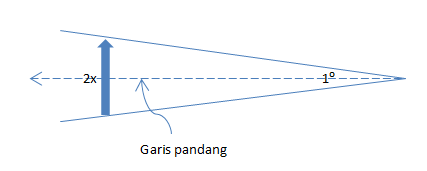
\includegraphics[width=0.6\textwidth]{gambar/2.png}
\end{figure}
\begin{eqnarray*}
\tan{0.5^{\circ}} &=& \frac{x}{110 \times 10^6}\\
x &=& 0.96 \times 10^6\\
2x &=& 1.92 \times 10^6 \quad \text{km}
\end{eqnarray*}


\vspace{0.5cm}
\question Radius bintang katai putih memenuhi hubungan
\begin{equation*}
R \approx \frac{R_{\odot}}{74} \left( \frac{M_{\odot}}{M} \right)^{1/3}
\end{equation*}
Jika bintang katai putih dianggap sebagai benda hitam sempurna serta memiliki massa 0,4 massa Matahari ($M_{\odot}$) dan temperatur efektif ($T_{\text{eff}}$) 10000 K, maka luminositas bintang (dalam satuan $L_{\odot}$) adalah
\begin{choices}
\choice $3,6 \times 10^{-4}$
\choice $3,0 \times 10^{-3}$
\choice $1,8 \times 10^{2}$
\choice $2,6 \times 10^{3}$
\choice $7,6 \times 10^{4}$
\end{choices}

\textit{Jawaban: B}\\
Untuk $M = 0,4 M_{\odot}$ kita peroleh
\begin{equation*}
R \approx \frac{R_{\odot}}{74} \left( \frac{M_{\odot}}{0.4 M_{\odot}} \right)^{1/3} = 0,0183 R_{\odot}
\end{equation*}
Luminositas bintang katai putih menjadi
\begin{eqnarray*}
\frac{L}{L_{\odot}} &=& \frac{\sigma T^4 4 \pi R^2}{\sigma T_{\odot}^4 4 \pi R_{\odot}^2}\\
\frac{L}{L_{\odot}} &=& \left( \frac{T}{T_{\odot}}\right)^{4} \left( \frac{R}{R_{\odot}} \right)^2\\
\frac{L}{L_{\odot}} &=& \left(\frac{10000}{5785}\right)^{4} \left( \frac{0,0183 R_{\odot}}{R_{\odot}} \right)^2\\
\frac{L}{L_{\odot}} &=& 2,99 \times 10^{-3}
\end{eqnarray*}


\vspace{0.5cm}
\question Misalkan $\mathcal{M}$ menyatakan magnitudo mutlak bolometrik sebuah bintang dan $\mathcal{P}$ menyatakan energi yang dipancarkan setiap detik (dalam satuan watt), maka berlaku hubungan
\begin{choices}
\choice $\mathcal{P} = 3,485 \times 10^{26} \times 10^{-0,4 \mathcal{M}}$
\choice $\mathcal{P} = 3,013 \times 10^{28} \times 10^{-0,4 \mathcal{M}}$
\choice $\log{\mathcal{P}} = 26,591 - 0,4 \mathcal{M}$
\choice $\log{\mathcal{P}} = 28,479 + 0,4 \mathcal{M}$
\choice $\mathcal{P} = -2,500 \log{\mathcal{M}}$
\end{choices}

\textit{Jawaban: B}\\
Magnitudo mutlak bolometrik terkait dengan luminositas dengan hubungan Pogson berikut
\begin{eqnarray*}
\mathcal{M} - \mathcal{M}_{\odot} &=& -2,5 \log{\frac{\mathcal{P}}{\mathcal{P}_{\odot}}}\\
\mathcal{M} - 4,72 &=& -2,5 \log{\frac{\mathcal{P}}{3,9 \times 10^{26}}}\\
\mathcal{M} - 4,72 &=& -2,5 \left( \log{\mathcal{P}} - 26,591 \right)\\
\log{\mathcal{P}} &=& 28,479 - 0,4 \mathcal{M}\\
\mathcal{P} &=& 3,013 \times 10^{28} \times 10^{-0,4 \mathcal{M}}
\end{eqnarray*}

\vspace{0.5cm}
\question Di antara lima pernyataan berikut, manakah pernyataan yang benar?  
\begin{choices}
\choice Urutan garis spektrum dalam kemunculam mereka pada bintang-bintang dengan menurunnya temperatur adalah: garis hidrogen yang sangat kuat, garis helium terionisasi, garis helium netral, garis logam netral, metal terionisasi, pita molekul titanium oksida
\choice Periode bintang ganda visual selalu lebih pendek daripada periode bintang ganda spektroskopi
\choice Bintang Sirius adalah bintang paling terang di langit, berarti ia merupakan bintang paling dekat dengan kita
\choice Bintang Alpha Centauri adalah bintang paling dekat dengan kita, berarti ia merupakan bintang paling terang di langit
\choice Sifat paling dasar dari bintang yang menentukan lokasinya di deret utama adalah massanya 
\end{choices}

\textit{Jawaban: E}\\
(A) Suhu mempengaruhi garis-garis spektrum yang terbentuk (karena bergantung pada tingkat energinya), untuk bintang diurutkan dari suhu yang paling tinggi harusnya adalah Helium terionisasi, Helium netral, metal terionisasi, Hidrogen netral, logam netral, dan pita molekul TiO. 

(B) Bintang ganda visual tentu jarak pisahnya harus lebar sehingga periodenya biasanya yang sangat panjang.

(C dan D) Terang bintang dilangit dipengaruhi terang intrinsik dan jaraknya.

(E) Semakin besar massa maka ia akan lahir sebagai bintang dengan menempati bagian deret utama makin ke kiri.



\vspace{0.5cm}
\question Perhatikan gambar di bawah yang merupakan skema kerja interferometer teleskop radio A dan B.

\begin{figure}[H]
\centering
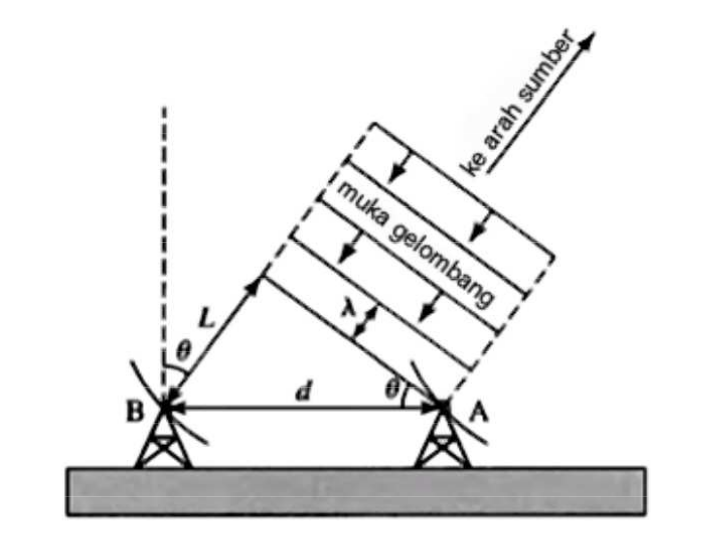
\includegraphics[width=0.4\textwidth]{gambar/6.png}
\end{figure}

Untuk mencapai resolusi sudut 1" dari objek astronomi yang di amati pada panjang gelombang 21 cm orde pertama, maka jarak minimal antara teleskop radio A dan B adalah
\begin{choices}
\choice 40,8 km 
\choice 41,3 km
\choice 42,3 km
\choice 43,3 km
\choice 44,3 km
\end{choices}

\textit{Jawaban: D}\\
Rumus resolusi sudut untuk teleskop dengan \textit{circular single aperture} (bukaan tunggal berbentuk lingkaran) dapat diturunkan (integral),
\begin{equation*}
\theta_{\text{res}} = \frac{1,22 \lambda}{D}
\end{equation*}
Untuk keperluan interferometer persamaan ini biasa didekati dengan
\begin{eqnarray*}
\theta_{\text{res}} &\approx& \frac{\lambda}{D}\\
\frac{1}{206265} \text{rad} &\approx&  \frac{21}{D}\\
D &\approx& 43.3 \times 10^5 \quad \text{cm} = 43.3 \quad \text{km}
%\frac{1}{206265} \text{rad} &=& \frac{1,22 \cdot 21}{D}\\
%D &=& 5,2845 \times 10^{6} \quad \text{cm} = 52,8 \quad \text{km}
\end{eqnarray*}

\vspace{0.5cm}
\question Rasi bintang zodiak yang dapat diamati pada saat bersamaan dengan peristiwa Gerhana Matahari Total 2016  di Indonesia, adalah
\begin{choices}
\choice Pisces
\choice Gemini
\choice Virgo
\choice Orion
\choice Canis
\end{choices}

\textit{Jawaban: A}\\
Seperti yang disebutkan pada soal nomor 8, gerhana Matahari terjadi pada tanggal 9 Maret 2016. Kita tahu rasi zodiak merupakan rasi-rasi bintang yang berada di ekliptika yang dilalui Matahari sepanjang tahun. Pada tanggal 9 Maret Matahari berada di antara rasi Pisces dan Aquarius, namun menurut  batasan wilayah rasi yang ditetapkan IAU, seharusnya Matahari masih berada di daerah rasi Aquarius. 

Posisi Matahari di rasi zodiak dapat dilihat pada kolom Astronomi di tabel berikut. Kalangan astrologi pecah menjadi dua kelompok, yang tetap menggunakan aturan di bawah (kolom astrologi) dan yang sesuai dengan posisi Matahari yang benar namun hanya melibatkan 12 rasi (tanpa Ophiuchus).

\begin{tabular}{|l|c|c|c|}
\hline 
\textbf{Rasi} & \textbf{Simbol} & \textbf{Astrologi (tropical)} & \textbf{Astronomi} \\ 
\hline 
Aries & $\aries$ & 21 Maret - 20 April & 19 April - 13 Mei \\ 
\hline 
Taurus & $\taurus$ & 21 April - 21 Mei &  14 Mei - 19 Juni\\ 
\hline 
Gemini & $\gemini$ & 22 Mei - 21 Juni & 20 Juni - 20 Juli \\ 
\hline 
Cancer & $\cancer$ & 22 Juni - 22 Juli & 21 Juli - 9 Agustus \\ 
\hline 
Leo & $\leo$ & 23 Juli - 22 Agustus & 10 Agustus - 15 September \\ 
\hline 
Virgo & $\virgo$ & 23 Agustus - 23 September & 16 September - 30 Oktober \\ 
\hline 
Libra & $\libra$ & 24 September - 23 Oktober & 31 Oktober - 22 November \\ 
\hline 
Scorpio & $\scorpio$ & 24 Oktober - 22 November & 23 November - 29 November \\ 
\hline 
Ophiuchus &  & - & 30 November - 17 Desember \\ 
\hline 
Sagittarius & $\sagittarius$ & 23 November - 21 Desember & 18 Desember - 18 Januari \\ 
\hline 
Capricorn & $\capricornus$ & 22 Desember - 20 Januari & 19 Januari - 15 Februari \\ 
\hline 
Aquarius & $\aquarius$ & 21 Januari - 19 Februari & 16 Februari - 11 Maret \\ 
\hline 
Pisces & $\pisces$ & 20 Februari - 20 Maret & 12 Maret - 18 April \\ 
\hline 
\end{tabular} 

Matahari paling lama berada di rasi Virgo (45 hari) dan paling sebentar berada di rasi Scorpio (7 hari) karena luas daerah rasi yang berbeda (ditetapkan IAU).

\vspace{0.5cm}
\question Pada tanggal 9 Maret 2016 pagi hari akan berlangsung Gerhana Matahari Total yang jalurnya melewati Indonesia, di antaranya kota Palembang, Palangkaraya, dan Palu. Perkiraan posisi Bulan dalam sistem koordinat ekuatorial ($\alpha, \delta$) pada saat tersebut adalah
\begin{choices}
\choice (23 jam, $-4^{\circ}$)
\choice (01 jam, $+4^{\circ}$)
\choice (23 jam, $-1^{\circ}$)
\choice (23 jam, $+1^{\circ}$)
\choice (24 jam, $+0^{\circ}$)
\end{choices}

\textit{Jawaban: A}\\
Pada saat terjadi gerhana Matahari total maka posisi Bulan di langit akan sama dengan posisi Matahari. Pada tanggal 20 Maret  $\alpha_{\odot} = 0^{h}$ dan $\delta_{\odot} = 0^{\circ}$, maka pada tanggal 9 Maret 
\begin{equation*}
\alpha_{\leftmoon} = \alpha_{\odot} \approx 24^h - 11 \cdot 4^m \approx 23^h 16^m
\end{equation*}
\begin{equation*}
\delta_{\leftmoon} = \delta_{\odot} \approx 23,5^{\circ} \sin{\left( \frac{-11}{365,25} 360^{\circ} \right)}\approx -4,4^{\circ}
\end{equation*}


\vspace{0.5cm}
\question Diketahui jarak rata-rata Bumi-Bulan adalah 384400 km dan periode orbit Bulan adalah 27,3 hari. Berapakah periode orbit sebuah satelit buatan yang mengitari Bumi pada ketinggian 96000 km jika orbitnya berupa lingkaran?
\begin{choices}
\choice 3,41 hari
\choice 3,76 hari
\choice 7,28 hari
\choice 10,40 hari
\choice 10,70 hari
\end{choices}

\textit{Jawaban: B}\\
Hukum Kepler III dapat ditulis ulang menjadi
\begin{equation*}
\frac{4 \pi^2 a^3}{T^2} = G(m_{1} + m_{2}) 
\end{equation*}
Untuk Bulan dan satelit yang mengorbit Bumi dapat kita abaikan massanya karena jauh lebih kecil dari massa Bumi. Kemudian dapat kita bandingkan keduanya
\begin{eqnarray*}
\frac{4 \pi^2 a^3/T^2}{4 \pi^2 a_{\leftmoon}^3/T_{\leftmoon}^2} &=& \frac{G M_{\oplus}}{G M_{\oplus}}\\
\left( \frac{T}{T_{\leftmoon}} \right)^2 &=& \left( \frac{a}{a_{\leftmoon}} \right)^3\\
\left( \frac{T}{27,3} \right)^2 &=& \left( \frac{102378}{384400} \right)^3\\
T &=& 3,753 \quad \text{hari}
\end{eqnarray*}





\vspace{1cm}
\textbf{Untuk empat soal berikut ini (No. 10\---13), jawablah}\\
A. jika 1, 2, dan 3 benar\\
B. jika 1 dan 3 benar\\
C. jika 2 dan 4 benar\\
D. jika 4 saja benar\\
E. jika semua benar\\

\vspace{0.5cm}
\question Jika atmosfer Bumi 50\% lebih rapat daripada keadaan saat ini, maka
\begin{enumerate}
\item Cahaya Matahari akan tampak lebih merah daripada keadaan sekarang, karena dengan bertambahnya kerapatan, akan lebih banyak cahaya pada panjang gelombang biru yang dihamburkan ke segala arah.
\item Cahaya yang sampai ke permukaan Bumi akan semakin tampak berwarna biru 
\item Cahaya yang sampai ke permukaan Bumi akan semakin tampak berwarna merah 
\item Cahaya Matahari akan tampak lebih biru daripada keadaan sekarang, karena dengan bertambahnya kerapatan, akan lebih banyak cahaya pada panjang gelombang merah yang dihamburkan ke segala arah.
\end{enumerate}

\textit{Jawaban: B}\\
Semakin tebal gas/debu maka efek pemerahan akan semakin kuat, panjang gelombang biru lebih banyak dihamburkan daripada merah.


\vspace{0.5cm}
\question Konstanta Hubble $H_0$ menyatakan laju pengembangan alam semesta saat ini. Karena kesalahan dalam penentuan jarak beberapa galaksi yang digunakannya, Edwin Hubble mendapatkan nilai sekitar 500 km/s/Mpc untuk $H_0$. Nilai yang diterima sekarang oleh para astronom berdasarkan berbagai pengukuran adalah 70 km/s/Mpc. Manakah pernyataan-pernyataan yang benar di bawah ini?
\begin{enumerate}
\item Laju pengembangan alam semesta menurut Hubble lebih cepat daripada seharusnya
\item Jarak galaksi-galaksi yang digunakan Hubble lebih jauh daripada seharusnya
\item Umur alam semesta menurut Hubble lebih muda daripada umur sebenarnya
\item Jika sejak \textit{Big Bang} alam semesta mengembang dengan laju konstan $H_0$, maka menurut Hubble ukuran alam semesta saat ini kurang lebih sepertujuh dari nilai yang diterima sekarang
\end{enumerate}

\textit{Jawaban: B}\\
(1) Konstanta Hubble menunjukkan kecepatan pengembangan alam semesta, (2) kesalahan Hubble dalam menentukan konstanta tersebut karena jarak galaksi yang digunakannya salah (lebih dekat dari yang seharusnya). Selain itu galaksi yang diamati semasa Hubble hanya galaksi-galaksi dekat saja (jika dibandingkan dengan hasil pengamatan modern). (3) Waktu Hubble yang sebanding dengan umur alam semesta dapat ditentukan dengan $1/H_0$. (4) Pernyataan 4 bisa benar apabila yang dimaksud adalah jarak Hubble ($c/H_0$), yang menunjukkan jarak dimana galaksi menjauhi kita dengan kecepatan cahaya akibat pengembangan alam semesta. Ukuran alam semesta yang sebenarnya tidak dapat diketahui hanya dengan konstanta Hubble.


\vspace{0.5cm}
\question Di antara empat pernyataan berikut, yang merupakan karakteristik materi antar bintang adalah
\begin{enumerate}
\item Dalam besaran massa, materi antar bintang tersusun atas Hidrogen, Helium, dan sedikit unsur berat 
\item Daerah hidrogen terionisasi (\textit{HII region}) terjadi akibat radiasi ultraviolet dari bintang panas di dekatnya
\item Materi antar bintang dapat terkait dengan pembentukan dan kematian bintang
\item Hanya ada satu kelompok daerah dalam materi antar bintang yaitu yang berhubungan dengan pembentukan bintang
\end{enumerate}

\textit{Jawaban: E}\\
Penjelasan untuk masing-masing pernyataan:
\begin{enumerate}
\item Ambigu; Jika yang dimaksud adalah diurutkan berdasarkan massa penyusun MAB, maka pernyataan 1 \textbf{benar}.
\item Ionisasi hidrogen dapat terjadi akibat foton UV yang energinya berkesesuaian (Pernyataan 2 \textbf{benar})
\item Bintang terbentuk di daerah materi antar bintang yang sangat rapat (\textit{molecular cloud}). MAB dapat diperbaharui oleh proses kematian bintang (\textit{supernovae}, \textit{planetary nebulae}) dan angin bintang (Pernyataan 3 \textbf{benar})
\item Ambigu; MAB terutama \textit{molecular cloud} memang terkait langsung dengan pembentukan bintang (Pernyataan 4 \textbf{benar})
\end{enumerate}


\vspace{0.5cm}
\question Yang merupakan karakteristik dalam proses pembentukan bintang adalah
\begin{enumerate}
\item Materi antar bintang yang melimpah dalam periode waktu yang lama, tidak selalu cukup untuk membentuk bintang
\item Proses pembentukan bintang dapat terjadi bila energi kinetik materi antar bintang lebih kecil dari setengah energi potensial gravitasi
\item Syarat terjadinya pembentukan bintang bergantung pada temperatur dan kerapatan partikel
\item Proses pembentukan bintang hanya dapat terjadi di daerah dengan konsentrasi debu tinggi
\end{enumerate}

\textit{Jawaban: A}\\
(1 dan 3) Proses runtuhnya awan dipengaruhi massa, kerapatan, dan temperatur (tekanan). Andaikan temperatur lingkungannya terlalu tinggi maka dimungkinkan awan untuk tidak runtuh menjadi bintang. (2) Temperatur adalah besaran statistik yang merepresentasikan energi kinetik rata-rata partikel dalam sistem, dari teorema virial diperoleh hubungan agar sistem dapat terikat dalam waktu lama maka $Ek = \frac{1}{2} E_p$. (4) Tidak selalu, jika begitu maka tidak ada bintang yang lahir ketika alam semesta masih dini (belum ada debu).


\vspace{1cm}
\textbf{Gunakan petunjuk ini untuk menjawab dua soal berikut (No. 14-15):}\\
A. Pernyataan pertama dan kedua benar serta memiliki hubungan sebab-akibat.\\
B. Pernyataan pertama dan kedua benar, tetapi tidak memiliki hubungan sebab-akibat.\\
C. Pernyataan pertama benar, sedangkan pernyataan kedua salah.\\
D. Pernyataan pertama salah, sedangkan pernyataan kedua benar\\
E. Kedua pernyataan salah.\\

\vspace{0.5cm}
\question Tepi bayangan sebuah objek yang dibentuk oleh sinar Matahari tidak tajam
\begin{center}
SEBAB
\end{center}
\noindent Jarak Bumi dari Matahari yang sangat jauh menyebabkan Matahari dianggap sebagai suatu sumber titik dan cahayanya mengalami difraksi atau pembelokan cahaya  

\textit{Jawaban: C}\\
Tepi bayangan yang dibentuk oleh sinar Matahari memang tidak tajam, hal ini akan terlihat lebih jelas apabila bendanya kita jauhkan dari layar. Penyebabnya adalah karena Matahari BUKAN benda titik (\textit{point source}). Cahaya yang berasal dari satu tepi dan tepi lainnya dari Matahari mengenai tepi benda dengan sudut yang sedikit berbeda, prosesnya sama seperti terbentuknya penumbra saat gerhana. 


\vspace{0.5cm}
\question Bulan mengorbit Bumi, sedangkan asteroid mengorbit Matahari.
\begin{center}
SEBAB
\end{center}
\noindent Ukuran asteroid lebih kecil daripada Bulan.

\textit{Jawaban: B}\\
Bulan mengorbit Bumi dan bersama-sama mereka mengorbit Matahari. Asteroid secara definisi adalah benda-benda ``kecil'' yang mengorbit Matahari. (pernyataan 1 \textbf{benar})
Ukuran asteroid memang lebih kecil daripada Bulan (pernyataan 2 \textbf{benar}), namun hal ini bukanlah penyebab dari perbedaan orbitnya dengan Bulan. 

Asteroid mengorbit Matahari karena pengaruh gravitasi Matahari lebih besar daripada planet, sedangkan Bulan mengorbit Bumi karena pada jarak itu pengaruh gravitasi Bumi lebih kuat daripada Matahari. Asteroid bisa saja berubah `mengorbit' planet ketika berpapasan dekat dengan planet.

\vspace{1cm}
\textbf{Soal Isian Singkat}

\vspace{0.5cm} 
\question Jarak antara dua sumber titik yang direkam oleh detektor pada bidang fokus sebuah teleskop bergantung pada $\ldots\ldots\ldots$

\textit{Jawaban: }\\
Panjang fokus teleskop DAN jarak pisah dua titik itu (jarak sudut). 

Pembentukan bayangan di bidang fokus dapat disederhanakan menggunakan prinsip \textit{pinhole camera} seperti berikut:
\begin{figure}[H]
\centering
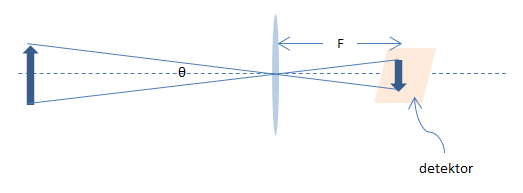
\includegraphics[width=0.7\textwidth]{gambar/16.png}
\end{figure}


\vspace{0.5cm}
\question Gugus bola IAU C0923 545 memiliki magnitudo semu $V = +13,0$ dan magnitudo mutlak $M_V = -4,15$. Gugus ini terletak 9,0 kpc dari Bumi, 11,9 kpc dari pusat Galaksi, dan sekitar 0,5 kpc di selatan bidang Galaksi. Besar serapan materi antar bintang per kpc yang kita amati ke arah IAU C0923 545 adalah $\ldots\ldots\ldots$

\textit{Jawaban: } 0.264 mag/kpc\\
Data jarak tidak \textit{self-consistent} antara jarak dari Bumi (9 kpc) dengan apabila menghitungnya menggunakan keterangan selanjutnya (serta data jarak pusat galaksi ke Bumi $\sim 8.5$ kpc).

Asumsi kita gunakan jarak dari Bumi 9 kpc sebagai jarak sebenarnya.
\begin{eqnarray*}
m - M &=& -5 + 5\log{d} + A_v\\
13 - (-4,15) &=& -5 + 5\log{9000} + A_v\\
A_v &=& 2,378 \quad \text{mag}\\
A_v &=& k \cdot d\\
A_v &=& k \cdot 9\\
k &=& 0.264 \quad \text{mag/kpc}\\
\end{eqnarray*}

\vspace{0.5cm}
\question Diduga terdapat sebuah planet X yang merupakan planet kesembilan di Tata Surya. Planet yang diperkirakan seukuran Uranus ini belum pernah teramati karena jaraknya yang jauh (20 kali jarak Matahari-Neptunus). \textit{Very Large Telescope} digunakan untuk mencari keberadaan planet tersebut dengan menggunakan teknik interferometer. Dengan detektor inframerah 20 mikron, jarak pisah minimal antar teleskop (\textit{baseline}) yang dibutuhkan untuk dapat menentukan ukuran planet secara langsung adalah sekitar $\ldots\ldots\ldots$

\textit{Jawaban: } 35,2 meter\\
Diameter sudut planet X 
\begin{eqnarray*}
\alpha &=& \frac{\text{diameter}}{\text{jarak}}\\
&=& \frac{51118}{20 \times 4,5043 \times 10^9 - 1,496 \times 10^8}\\
&=& 5,68 \times 10^{-7} \quad \text{rad}
\end{eqnarray*}

Resolusi minimal yang diperlukan membutuhkan $\theta_{\text{res}} \leq \alpha$
\begin{eqnarray*}
\theta_{\text{res}} &\approx& \frac{\lambda}{D} \qquad \longrightarrow \quad  \text{interferometer}\\
D &=& \frac{2 \times 10^{-5}}{5,68 \times 10^{-7}}\\
D &=& 35,2 \quad \text{meter}
\end{eqnarray*}


\vspace{0.5cm}
\question Salah satu sumber pemancar radio terkuat di langit setelah Matahari dan Cassiopeia A (sisa supernova yang relatif dekat) adalah Galaksi Cygnus A. Pada panjang gelombang 0,75 cm, rapat fluks spektral yang diukur oleh teleskop radio dengan diameter 25 m adalah 4500 Jy (jansky). Dengan menganggap efisiensi teleskop radio 100\% dan lebar pita frekuensi adalah 5 MHz, daya total yang dideteksi penerima adalah sebesar $\ldots\ldots\ldots$ watt.  

\textit{Jawaban: } $1,1 \times 10^{-13}$\\

1 Jy = $10^{-26}$ watt m$^{-2}$ Hz$^{-1}$

Total daya yang diterima teleskop adalah
\begin{eqnarray*}
P_{\text{total}} &=& F \times \text{Area} \times \text{bandwidth} \\
&=& (4500 \times 10^{-26}) \text{  watt m}^{-2} \text{Hz}^{-1} \times (\frac{1}{4} \cdot \pi \cdot 25^2) \text{  m}^2 \times (5 \times 10^6) \text{  Hz}\\
&=& 1,1 \times 10^{-13} \quad \text{watt}
\end{eqnarray*}


\vspace{0.5cm}
\question Jika Matahari berevolusi menjadi bintang raksasa merah dengan ukuran 100 kali jejari Matahari saat ini dan temperaturnya menjadi 3200 $^{\circ}$C, maka magnitudo semu Matahari raksasa adalah $\ldots\ldots\ldots$

\textit{Jawaban: } -34,56\\
Asumsikan kita melihatnya dari Bumi (jarak 1 sa).
\begin{eqnarray*}
m - m_0 &=& -2,5 \log{\frac{E}{E_0}}\\
m - m_0 &=& -2,5 \log{\frac{L}{L_0}}\\
m - m_0 &=& -2,5 \log{\left( \left(\frac{R}{R_0}\right)^2 \left(\frac{T}{T_0}\right)^4 \right)}\\
m - (-26,78) &=& -2,5 \log{\left( \left(\frac{100 R_0}{R_0}\right)^2 \left(\frac{3473}{5785}\right)^4 \right)}\\
m &=& -34,56 
\end{eqnarray*}

\vspace{1cm}
\textbf{Soal Esai}

\vspace{0.5cm}
\question Pada pukul 18:00, tinggi dan azimuth Bulan adalah $+39^{\circ}$ dan $196^{\circ}$, sedangkan tinggi dan azimuth Saturnus adalah $+34^{\circ}$ dan $210^{\circ}$. Jika Bulan dan Saturnus dianggap benda titik, hitunglah jarak pisah kedua benda tersebut dalam satuan derajat!  

\textit{Jawaban: }\\
\begin{eqnarray*}
\cos{x} &=& \cos{(90^{\circ} - 39^{\circ})}\cos{(90^{\circ} - 34^{\circ})} + \sin{(90^{\circ} - 39^{\circ})}\sin{(90^{\circ} - 34^{\circ})}\cos{(210^{\circ} - 196^{\circ})}\\
\cos{x} &=& \sin{39^{\circ}} \sin{34^{\circ}} + \cos{39^{\circ}} \cos{34^{\circ}} \cos{14^{\circ}}\\
\cos{x} &=& 0.97705673352\\
x &=& 12,3^{\circ}
\end{eqnarray*}


\vspace{0.5cm}
\question Dengan teleskop Hubble, astronom dapat mengamati bintang seperti Matahari pada jarak 100 kpc. Bintang-bintang Cepheid yang paling terang memiliki kecerlangan intrinsik 30000 kali lebih besar daripada Matahari. Jika serapan materi antar bintang diabaikan, tentukanlah jarak Cepheid terjauh yang dapat diamati teleskop Hubble!

\textit{Jawaban: }\\
Keterangan bahwa teleskop Hubble dapat melihat bintang sekelas Matahari hingga jarak 100 kpc dapat kita gunakan sebagai batasan maksimum. Untuk cepheid yang lebih terang tentu jarak maksimumnya bisa lebih jauh. Fluks energi yang diterima dari kedua benda harusnya sama pada jarak maksimumnya masing-masing sebagai batas fluks minimal yang masih terdeteksi oleh Hubble,
\begin{eqnarray*}
\frac{L_{\odot}}{4 \pi d_{\odot}^2} &=& \frac{L_{\text{ceph}}}{4 \pi d_{\text{ceph}}^2}\\
\left( \frac{d_{\text{ceph}}}{d_{\odot}} \right)^2 &=& \frac{L_{\text{ceph}}}{L_{\odot}} = 30000\\
\frac{d_{\text{ceph}}}{d_{\odot}} &=& 173,2 \\
d_{\text{ceph}} &=& 17320,5 \quad \text{kpc} = 17,32 \quad \text{Mpc}  
\end{eqnarray*}


\vspace{0.5cm}
\question Gunung Olympus yang memiliki tinggi 25 km adalah gunung tertinggi di Mars sekaligus tertinggi di Tata Surya. Bahkan tiga kali lebih tinggi dari gunung Himalaya. Untuk mengetahui mengapa planet Mars dapat memiliki gunung tertinggi di Tata Surya, maka
\begin{enumerate}[(a)]
\item Hitunglah tinggi maksimum gunung di Bumi bila gunung dianggap berbentuk kerucut! Ambillah nilai batas elastisitas kerak Bumi sebesar $3 \times 10^8$ N/m$^{2}$!
\item Jelaskan mengapa gunung tertinggi di Tata Surya dapat berada di planet Mars!
\end{enumerate} 

\textit{Jawaban: }\\
\begin{enumerate}[a.]
\item Batas elastisitas adalah nilai tekanan di mana suatu benda tidak dapat kembali lagi seperti semula (terjadi deformasi permanen). Sebagai contoh sederhana andaikan kita memiliki meja kayu, tentu ada batasan tekanan dari benda yang kita taruh di atasnya sehingga maja kayu tersebut akan patah. Andaikan meja tersebut adalah kerak Bumi dengan nilai limit elastisitas $3 \times 10^8$ N/m$^{2}$, maka kita dapat memperkirakan tinggi maksimum ``benda'' yang berada di atasnya (gunung), apabila kita mengetahui tekanan yang ia berikan ke kerak Bumi.

\begin{figure}[H]
\centering
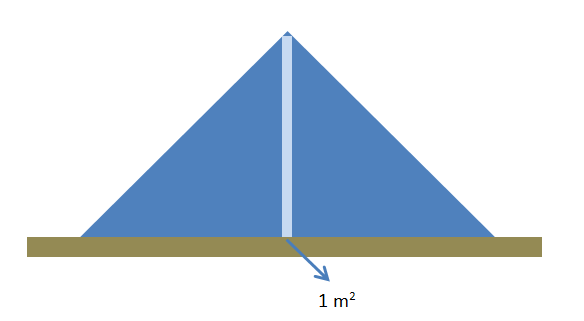
\includegraphics[width=0.6\textwidth]{gambar/mount.png}
\end{figure}

Bagian tengah gunung seperti digambarkan di atas (biasanya bagian paling tinggi) adalah bagian dengan berat terbesar yang ditahan oleh kerak Bumi. Jika berat maksimum yang ditahan Bumi per meter perseginya adalah $3 \times 10^8$ N, maka hal ini berkesesuaian dengan tinggi

\begin{eqnarray*}
W &=& M \cdot g\\
W &=& \rho \cdot V \cdot g\\
3 \times 10^8 &=& 5520 \cdot 1 \quad \text{m}^2 \cdot \text{tinggi}_{\text{maks}} \cdot 9.8 \\
\text{tinggi}_{\text{maks}} &=& 5545 \quad \text{m}
\end{eqnarray*}

Nilai kerapatan yang digunakan di atas adalah kerapatan rata-rata Bumi dari daftar konstanta massa dan jari-jari Bumi. Seharusnya nilai kerapatan yang digunakan adalah nilai kerapatan kerak Bumi yang lebih rendah. Tinggi gunung Everest adalah 8848 meter.


\item Percepatan gravitasi yang lebih kecil menyebabkan berat menjadi lebih kecil. Jika kerapatan Mars dan batas elastisitas permukaan Mars kira-kira sama dengan Bumi maka tentu saja gunung di Mars bisa dimungkinkan lebih tinggi dari gunung di Bumi. 

Percepatan gravitasi di permukaan di Mars dapat dihitung
\begin{equation*}
g = \frac{GM}{R^2} = 3,7 \text{m/s}^2
\end{equation*}
Sedikit lebih besar dari sepertiga percepatan gravitasi di Bumi.

Selain itu aktivitas dipermukaan planet Mars relatif lebih kecil dibanding planet terestrial lain seperti Bumi dan Venus (aktivitas ini berupa aktivitas atmosfer dan vulkanik), sehingga memungkinkan struktur lebih tinggi tersebut dapat bertahan.

\end{enumerate}


\vspace{0.5cm}
\question Di Galaksi, sebuah proton berenergi $10^7$ eV melintasi medan magnet antar bintang yang homogen ($B = 3 \times 10^{-10}$ T) dalam arah tegak lurus sehingga bergerak melingkar. Proton tersebut memiliki laju awal $v \ll c$ (non relativistik).
\begin{enumerate}[(a)]
\item Hitunglah momentum linear proton tersebut!
\item Hitunglah radius gerak melingkar proton (\textit{gyroradius}) dan frekuensi sudut yang dihasilkan!
\item Gambarkan arah gerak dan lintasan proton jika proton membentuk sudut tertentu (dengan sudut sekitar $30^{\circ}$) terhadap garis medan magnet!
\end{enumerate}

\textit{Jawaban: }\\
\begin{enumerate}[a.]
\item Momentum linear proton
\begin{eqnarray*}
E_k &=& \frac{p^2}{2m}\\
p &=& \sqrt{10^7 \cdot 1.6 \times 10^{-19} \cdot 2 \cdot 1,6726 \times 10^{-27}}\\
p &=& 7,316 \times 10^{-20} \quad \text{kg m/s}
\end{eqnarray*}
Kecepatannya dapat dihitung yang sebenarnya cukup relativistik yaitu 0,146 c. 

Karena proton mengalami gerak melingkar (terdapat percepatan sentripetal) maka ia akan menghasilkan radiasi yang disebut dengan radiasi \textit{cyclotron}. Jika kecepatannya \textit{hyperrelativistic} ($v \sim c$) maka akan menghasilkan radiasi \textit{synchrotron}.

\item Radius gerak melingkar dapat ditentukan dengan
\begin{eqnarray*}
m\frac{v^2}{r} &=& q v \times B = q v B\\
r &=& \frac{mv}{qB} = \frac{p}{qB} = \frac{7,316 \times 10^{-20}}{1,6 \times 10^{-19} \cdot 10^{-10}}\\
r &=& 4,5725 \times 10^{8} \quad \text{m}
\end{eqnarray*}


\item Gerak proton jika membentuk sudut tidak tegak lurus (dan tidak sejajar) maka menjadi spiral seperti berikut,

\begin{figure}[H]
\centering
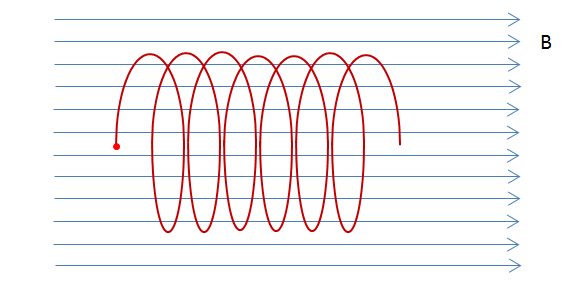
\includegraphics[width=0.6\textwidth]{gambar/spiral.png}
\end{figure}

Hal itu terjadi karena yang terpengaruh oleh medan magnet hanya komponen kecepatan yang arahnya tegak lurus dengannya ($q v \times B = qvB \sin{\theta}$ ). Gambar di atas tidak terlalu merepresentasikan dengan baik dari data sudut $30^{\circ}$ (harusnya lebih melar ke samping).


\end{enumerate}

\vspace{0.5cm}
\question Pada akhir Januari 2016 terjadi fenomena langka yaitu 5 planet klasik tampak berparade di langit fajar. Merkurius tampak di arah Timur, diikuti Venus, Saturnus, Mars, dan Jupiter di sebelah Barat. Jika jarak sudut Jupiter dan Merkurius adalah $100^{\circ}$ sementara sudut elongasi Merkurius dari Matahari adalah $15^{\circ}$, hitunglah jarak antara Jupiter dan Merkurius dalam satuan astronomi! Anggap orbit kelima planet berada dalam satu bidang!

\textit{Jawaban: }\\
Sebelumnya dapat kita hitung jarak Bumi-Merkurius (EM) dan jarak Bumi-Jupiter (EJ) saat itu

\begin{eqnarray*}
SM^2 &=& ES^2 + EM^2 - 2 \cdot ES \cdot EM \cdot \cos{15^{\circ}}\\
0 &=& EM^2 - 1,93185 EM + 0,8501544\\
\end{eqnarray*}
Solusi persamaan kuadrat tersebut adalah
\begin{equation*}
EM_{12} = \frac{1,93185 \pm \sqrt{1,93185^2 - 4 \cdot 1 \cdot 0,8501544}}{2 \cdot 1}
\end{equation*}
\begin{equation*}
EM_1 = EM' = 1,2538 \quad \text{dan} \quad EM_2 = EM = 0,6781 
\end{equation*}

Terlihat bahwa terdapat dua solusi positif dari persamaan kuadrat ini yang memang wajar karena ada dua posisi yang mungkin seperti ditunjukkan pada gambar berikut ($M$ dan $M'$):

\begin{figure}[H]
\centering
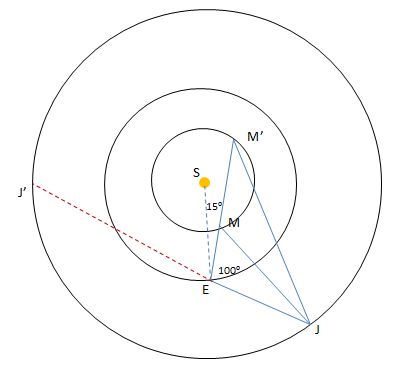
\includegraphics[width=0.6\textwidth]{gambar/25.png}
\end{figure}

Jarak Jupiter dapat ditentukan dengan cara yang sama 
\begin{eqnarray*}
SJ^2 &=& ES^2 + EJ^2 - 2 \cdot ES \cdot EJ \cos{115^{\circ}}\\
0 &=& EJ^2 + 0,8452365 EJ - 26,0685102\\
EJ_1 &=& 4,700576 \quad \text{dan} \quad EJ_2 =  -5,5458
\end{eqnarray*}
di mana hanya ada satu nilai positif yang dapat kita gunakan (nilai negatif menunjukkan posisi Jupiter yang berseberangan ($J'$), sehingga tidak sesuai soal).

Jarak Jupiter dan Merkurius dapat ditentukan dengan cara yang sama pula menghasilkan
\begin{eqnarray*}
MJ^2 &=& EM^2 + EJ^2 - 2 \cdot EM \cdot EJ \cos{100^{\circ}}\\
MJ &=& 4,86438 \quad \text{sa}\\
M'J^2 &=& EM'^2 + EJ^2 - 2 \cdot EM' \cdot EJ \cos{100^{\circ}}\\
M'J &=& 5,07092 \quad \text{sa}
\end{eqnarray*}

Hasil akhirnya ada dua nilai jarak yang memenuhi, yakni 4,864 dan 5,071 sa.

- Cara yang lain dapat dilakukan dengan menghitung sudut di Matahari antara Merkurius dan Jupiter saat itu, kemudian dapat kita hitung jarak keduanya. 

- Jika menggunakan rumus sinus ingat bahwa nilai $\arcsin$ ada dua, kalkulator biasanya hanya menunjukkan satu angka.

\end{questions}

\newpage
\center \textbf{Daftar Konstanta}

\begin{table}[ht]
\centering
\label{tab:konstanta01}
\renewcommand{\arraystretch}{1.3}
\begin{tabular}{|l|c|c|}
\hline
\textbf{Nama Besaran} & \textbf{Notasi} & \textbf{Harga}\\
\hline
\hline
Satuan astronomi & au & $1,49597870 \times 10^{11}$ m\\
\hline
Parsek & pc & $3,0857 \times 10^{16}$ m\\
\hline
Tahun Cahaya & ly & $0,9461 \times 10^{16}$ m\\
\hline
Tahun Sideris &  & 365,2564 hari\\
\hline
Tahun Tropik &  & 365,2422 hari\\
\hline
Tahun Gregorian &  & 365,2425 hari\\
\hline
Tahun Julian &  & 365,2500 hari\\
\hline
Periode sinodis Bulan (\textit{synodic month}) &  & 29,5306 hari\\
\hline
Periode sideris Bulan (\textit{sidereal month}) &  & 27,3217 hari\\
\hline
Hari Matahari rerata (\textit{mean solar day}) &  & 24$^{j}$ 3$^{m}$ 56$^{d}$,56\\
\hline
Hari sideris rerata (\textit{mean sidereal day}) &  & 23$^{j}$ 56$^{m}$ 4$^{d}$,00\\
\hline
Massa Matahari & $M_{\odot}$ & $1,989 \times 10^{30}$ kg\\
\hline
Jejari Matahari & $R_{\odot}$ & $6,96 \times 10^{8}$ m\\
\hline
Temperatur efektif Matahari & $T_{\text{eff} \odot}$ & 5785 K\\
\hline
Luminositas Matahari & $L_{\odot}$ & $3,9 \times 10^{26}$ W\\
\hline
Magnitudo semu visual Matahari & $V$ & -26,78\\
\hline
\multirow{2}{*}{Indeks warna Matahari} & $B - V$ & 0,62\\ \cline{2-3}
                                       & $U - B$ & 0,10\\
\hline
Magnitudo mutlak visual Matahari & $M_{V}$ & 4,79\\
\hline
Magnitudo mutlak biru Matahari & $M_{B}$ & 5,48\\
\hline
Magnitudo mutlak bolometrik Matahari & $M_{bol}$ & 4,72\\
\hline
Massa Bulan & $M_{\leftmoon}$ & $7,348 \times 10^{22}$ kg\\
\hline
Jejari Bulan & $R_{\leftmoon}$ & 1738000 m\\
\hline
Jarak rerata Bumi-Bulan & & 384399000 m\\
\hline
Konstanta Hubble & $H_{0}$ & 69,3 km/s/Mpc\\
\hline
Jansky & Jy & $10^{-26}$ watt m$^{-2}$ Hz$^{-1}$\\
\hline
\end{tabular} 
\end{table}

\newpage
\begin{table}[ht]
\centering
\label{tab:konstanta02}
\renewcommand{\arraystretch}{1.4}
\begin{tabular}{|c|c|c|c|c|c|}
\hline
\multirow{3}{*}{\textbf{Objek}} & \multirow{3}{*}{\textbf{Massa}} & \textbf{Jejari} & \multirow{3}{*}{\textbf{P}$_{\text{rotasi}}$} & \multirow{3}{*}{\textbf{P}$_{\text{sideris}}$} & \textbf{Jarak rerata} \\
& & \textbf{ekuatorial} & & & \textbf{ke Matahari} \\
& \textbf{(kg)} & \textbf{(km)} & & \textbf{(hari)} & ($10^{3}$ \textbf{km})\\
\hline
\hline
Merkurius & $3,3 \times 10^{23}$ & 2440 & 58,646 hari & 87,9522 & 57910 \\
\hline
Venus & $4,87 \times 10^{24} $ & 6052 & 243,019 hari & 224,701 & 108200 \\
\hline
Bumi & $5,97 \times 10^{24}$ & 6378 & $23^{j}56^{m}4^{d},1$ & 365,25 & 149600\\
\hline
Mars & $6,42 \times 10^{23}$ & 3397 & $24^{j}37^{m}22^{d},6$ & 686,9257 & 227940\\
\hline
Jupiter & $1,90 \times 10^{27}$ & 71492 & $9^{j}55^{m}30^{d}$ & 4330,5866 & 778330\\
\hline
Saturnus & $5,69 \times 10^{26}$ & 60268 & $10^{j}39^{m}22^{d}$ & 10746,9334 & 1429400\\
\hline
Uranus & $8,66 \times 10^{25}$ & 25559 & $17^{j}14^{m}24^{d}$ & 30588,5918 & 2870990\\
\hline
Neptunus & $1,03 \times 10^{26}$ & 24764 & $16^{j}6^{m}36^{d}$ & 59799,8258 & 4504300\\
\hline
\end{tabular}
\end{table}

\begin{table}[ht]
\centering
\label{tab:konstanta03}
\renewcommand{\arraystretch}{1.4}
\begin{tabular}{|l|c|c|}
\hline
\textbf{Nama konstanta} & \textbf{Simbol} & \textbf{Harga}\\
\hline
\hline
Kecepatan cahaya & $c$ & $2,99792458 \times 10^{8}$ m/s\\
\hline
Konstanta gravitasi & $G$ & $6,673 \times 10^{-11}$ m$^{3}$/kg/s$^{2}$\\
\hline
Konstanta Planck & $h$ & $6,6261 \times 10^{-34}$ Js\\
\hline
Konstanta Boltzmann & $k$ & $1,3807 \times 10^{-23}$ J/K\\
\hline
Konstanta kerapatan radiasi & $a$ & $7,5659 \times 10^{-16}$ J/m$^3$/K$^4$\\
\hline
Konstanta Stefan-Boltzmann & $\sigma$ & $5,6705 \times 10^{-8}$ Watt/m$^2$/K$^4$\\
\hline
Muatan elektron & $e$ & $1,6022 \times 10^{-19}$ C\\
\hline
Massa elektron & $m_e$ & $9,1094 \times 10^{-31}$ kg\\
\hline
Massa proton & $m_p$ & $1,6726 \times 10^{-27}$ kg\\
\hline
Massa neutron & $m_n$ & $1,6749 \times 10^{-27}$ kg\\
\hline
Massa atom $_{1}H^{1}$ & $m_H$ & $1,6735 \times 10^{-27}$ kg\\
\hline
Massa atom $_{2}He^{4}$ & $m_{He}$ & $6,6465 \times 10^{-27}$ kg\\
\hline
Massa inti $_{2}He^{4}$ &  & $6,6430 \times 10^{-27}$ kg\\
\hline
Konstanta gas & $R$ & 8,3145 J/K/mol\\
\hline
\end{tabular} 
\end{table}

\vspace{1cm}
\begin{flushright}
Solusi ini dapat diperoleh di \href{http://ridlow.wordpress.com}{http://ridlow.wordpress.com}
\end{flushright}
\end{document}
